\documentclass[a4paper, 12pt]{article}
\usepackage{graphicx}  
\usepackage{listings}  
\usepackage{xcolor}    

\lstset{
    frame=single,
    breaklines=true,
    basicstyle=\ttfamily\small,
    keywordstyle=\color{blue},
    commentstyle=\color{gray},
    stringstyle=\color{red},
    numbers=left,
    numberstyle=\tiny,
    stepnumber=1,
    numbersep=5pt,
    language=Python
}

\title{Practical Work 1: TCP File Transfer}
\author{Group Members: \\[0.2cm]
- Member 1 Le Quoc Trung \\ 
- Member 2 Nguyen Kien Trung \\
- Member 3 Nguyen Dinh Tung \\
- Member 4 Nguyen Huy Tung \\
- Member 5 Nguyen Duc Bao Minh \\
}
\date{\today}

\begin{document}

\maketitle

\section{Introduction}
This report describes the implementation of a file transfer system using TCP/IP in a Command-Line Interface (CLI). The system is composed of a server and a client, which communicate using sockets to transfer a file from the client to the server. The goal is to demonstrate a basic implementation of file transfer over TCP, based on a provided chat system.

\section{Protocol Design}
The file transfer protocol involves the following steps:
\begin{enumerate}
    \item The server binds to a specific port and listens for incoming connections.
    \item The client connects to the server and sends metadata about the file (file name and file size).
    \item The server acknowledges and prepares to receive the file.
    \item The client sends the file in chunks.
    \item The server writes the received chunks to a file on disk.
    \item Both client and server close the connection after the transfer is complete.
\end{enumerate}

\begin{figure}[h]
    \centering
    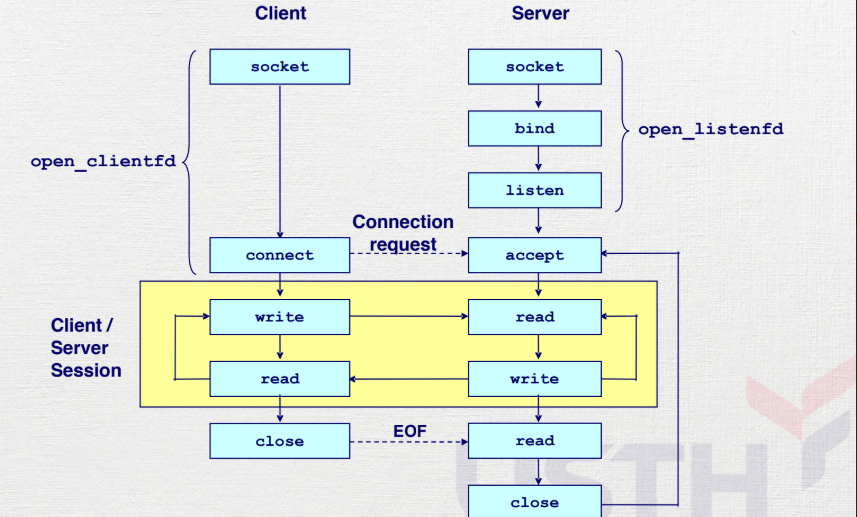
\includegraphics[width=0.8\textwidth]{chill.png}
    \caption{Protocol Design for TCP File Transfer}
    \label{fig:protocol}
\end{figure}

\section{System Organization}
The system consists of two main components:
\begin{itemize}
    \item \textbf{Server:} Responsible for receiving and saving the file.
    \item \textbf{Client:} Responsible for sending the file to the server.
\end{itemize}

\begin{figure}[h]
    \centering
    \includegraphics[width=0.8\textwidth]{1.png}
    \caption{System Organization of Server and Client}
    \label{fig:architecture}
\end{figure}

\section{Implementation}
Below are the key code snippets for implementing the TCP file transfer:

\subsection{Server Code}
\begin{lstlisting}[caption=Server Code]
import socket

def start_server(host='127.0.0.1', port=5000):
    server_socket = socket.socket(socket.AF_INET, socket.SOCK_STREAM)
    server_socket.bind((host, port))
    server_socket.listen(1)
    print(f"Server listening on {host}:{port}")

    conn, addr = server_socket.accept()
    print(f"Connection established with {addr}")

    with conn:
        file_name = conn.recv(1024).decode()
        file_size = int(conn.recv(1024).decode())
        print(f"Receiving file: {file_name}, Size: {file_size} bytes")

        with open(file_name, 'wb') as file:
            received = 0
            while received < file_size:
                data = conn.recv(1024)
                if not data:
                    break
                file.write(data)
                received += len(data)
                print(f"Received {received}/{file_size} bytes")
    
    server_socket.close()
    print("File transfer complete, server closed.")

if __name__ == "__main__":
    start_server()
\end{lstlisting}

\subsection{Client Code}
\begin{lstlisting}[caption=Client Code]
import socket
import os

def send_file(file_path, host='127.0.0.1', port=5000):
    client_socket = socket.socket(socket.AF_INET, socket.SOCK_STREAM)
    client_socket.connect((host, port))

    file_name = os.path.basename(file_path)
    file_size = os.path.getsize(file_path)

    client_socket.send(file_name.encode())
    client_socket.send(str(file_size).encode())
    print(f"Sending file: {file_name}, Size: {file_size} bytes")

    with open(file_path, 'rb') as file:
        while chunk := file.read(1024):
            client_socket.send(chunk)
            print(f"Sent {len(chunk)} bytes")
    
    client_socket.close()
    print("File transfer complete, client closed.")

if __name__ == "__main__":
    file_path = "path/to/your/file.txt"
    send_file(file_path)
\end{lstlisting}

\section{Roles and Responsibilities}
\begin{itemize}
    \item \textbf{Member 1:} Implemented the server-side code and ensured robust error handling.
    \item \textbf{Member 2:} Developed the client-side code and tested file transfers.
    \item \textbf{Member 3:} Documented the protocol design and system organization in the report.
\end{itemize}

\section{Conclusion}
This practical work demonstrates a simple 1-1 file transfer system over TCP/IP. The implementation uses Python's socket library to establish communication between a client and a server. The system successfully transfers files, showcasing the use of fundamental socket programming concepts.

\end{document}
